

%interpretation of results


Through simulation studies, I have tested three potential methods for reducing the bias seen in the \parencite{michelot_langevin_2019} estimator for the Langevin process. The result of the first of these studies is shown in figure~\ref{fig:EKF_thin_boxplot}. This figure shows that the likelihood obtained by using the Extended Kalman filter performs slightly worse than the Euler-Maruyama method for the parameter $\beta_1$ and $\beta_2$. A reason for this might be that the method was tested in a scenario where the Brownian motion is much larger than the drift in the Langevin process, which is what one might expect in an animal setting. This makes the predict steps of the extended Kalman filter undershoot the steps of the Langevin process. In turn this leads to an error, which is compounded every time the predict step is performed. If the position used in the predict step is wrong, the prediction of the covariance using the curvature of the covariates also becomes wrong. To see how the extended Kalman filter works in practice I used the covariates from earlier and plotted the predict steps of the Langevin process together with steps of the extended Kalman filter, and the 90\% confidence level using the predicted covariance. The results are shown in figure~\ref{fig:EKF high diffusion}. 


\begin{figure}[H]
    \centering
    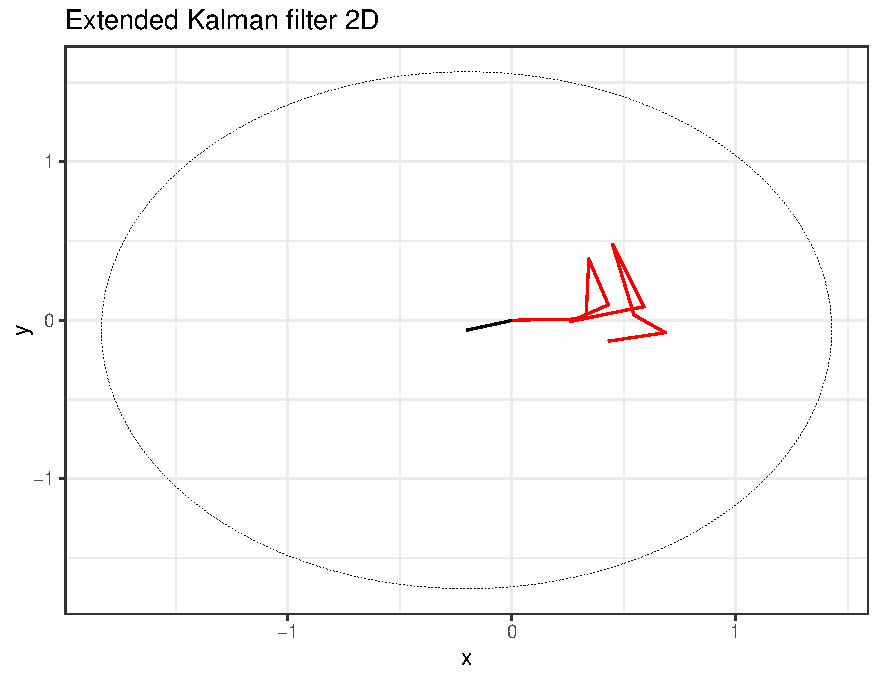
\includegraphics[width=\linewidth]{Images/discussion/EKF high diffusion path.pdf}
    \caption[Extended Kalman filter]{Plot of extended Kalman filter state estimates. The black line shows the predicted state estimates over a time grid from 0 to 0.1, with increments 0.01. The dotted elipse shows the 90\% confidence level set of the final predicted state, and the red line show the Langevin process that is beeing estimated. The parameters used are the same for the Langevin process and the EKF}
    \label{fig:EKF high diffusion}
\end{figure}

Figure~\ref{fig:EKF high diffusion} shows that there is little correspondence between the path of the predictions made by the extended Kalman filter and the Langevin process. In this case the paths have ended up going in almost opposite directions. This happens because the Langevin process pictured is dominated by randomness, which also means that the Langevin path is much longer than the path from the extended Kalman filter. Since the intermediate values of extended Kalman filter do not approximate the intermediate values of the Langevin process wee, doing multiple steps of the extended Kalman filter might not make an improvement to the estimate
The extended Kalman filter might work better. Using intermediate predict steps in the extended Kalman filter might work better in scenarios where the diffusion is maller and the drift larger, since the predictions would deviate less from the true values of the Langevin process.






%are the results meaningful









%what went well, what are constraints








%applications









%what is unknown or needs more exploration





Animal movement can be time dependent. This model would not allow for such adjustments since that would make the stationary distribution hard to find, meaning the method could not be used to incorporate other types of data.



These methods might not work as well in a setting where the drift dominates, since the path might go in curves which is hard for the brownian bridges to simulate. Though, in cases where the drift dominates, it is usually easier to estimate the parameters.


adding curvature to the brownian bridges could maybe improve the model


There should be done a study of the effect of observation error on the estimates using brownian bridge importance sampling

the estimates can be tested using the likelihood ratio test


In reality, the occurrence data is not collected without bias

the step interval of the track data might significantly affect the parameter estimates

Animal movement can be time dependent. This model would not allow for such adjustments since that would make the stationary distribution hard to find, meaning the method could not be used to incorporate other types of data.

An animal movement model that allows for point process integration can be done much more easily using the metropolis hastings algorithm

i could have tested the EKF for more values